%=======================================================================
% cap5_resultados.tex — Resultados
%=======================================================================

Este capítulo reporta los resultados de las fases de modelado y evaluación.
Sigue el orden de los objetivos específicos: los clasificadores de audio e
imagen por separado (OE2), su fusión multimodal (OE2), los \textit{baselines}
de referencia (OE4), el modelo de distribución frente a MaxEnt (OE3) y el
prototipo que integra los modelos. Cierra con una síntesis frente a los
objetivos y las métricas de costo computacional (OE5). Los hiperparámetros
completos están en el Apéndice~\ref{ape:hiperparametros} y las métricas por
especie en el Apéndice~\ref{ape:metricas}.

%-----------------------------------------------------------------------
\section{Protocolo experimental}\label{sec:protocolo}

Todos los experimentos usan PyTorch \citep{paszke2019pytorch}, los modelos
preentrenados de \texttt{timm} y Hugging Face, y los modelos clásicos de
\texttt{scikit-learn}, con semilla fija en particiones y entrenamientos. Las
métricas son las definidas en la \secref{sec:teoria-metricas}:
\textit{accuracy}, F1 macro y AUC-ROC para la identificación, y AUC-ROC por
especie para la distribución. Se usan tres protocolos de evaluación, que la
\secref{sec:teoria-inferencia} describe en detalle:

\begin{itemize}[leftmargin=*, itemsep=2pt]
  \item \textbf{Audio: ventana única y agregado por grabación.} Los modelos
        de audio no clasifican la grabación entera sino ventanas cortas
        (\SI{5}{\second} en la CNN, \SI{10}{\second} en el AST). En el
        protocolo de \emph{ventana única} se clasifica solo la ventana central
        de cada grabación. En el protocolo \emph{agregado} se clasifican hasta
        12 ventanas de \SI{5}{\second} en la CNN (hasta 8 de \SI{10}{\second}
        en el AST) repartidas a lo largo de la grabación y se promedian sus
        probabilidades antes de decidir. El agregado es la métrica
        operacional, pues en uso real se clasifica la grabación entera. Los
        valores de ventana única de las tablas de este capítulo son los que
        entrega el \textit{script} de entrenamiento sobre la ventana central
        de cada grabación.
  \item \textbf{Imagen: recorte central y TTA.} En el protocolo base la
        fotografía se reduce y se recorta un cuadrado central de \SI{384}{px},
        que es lo que ve el modelo. En la aumentación en tiempo de prueba
        (TTA) el modelo ve diez versiones de la misma fotografía (recortes de
        las cuatro esquinas y del centro, y sus reflejos horizontales) y se
        promedian las diez probabilidades, lo que suaviza errores debidos al
        encuadre.
  \item \textbf{Fusión: pareo por especie.} Como las grabaciones y las
        fotografías no corresponden a los mismos individuos, cada grabación
        del conjunto de prueba de audio se empareja al azar con una fotografía
        del conjunto de prueba de imagen de la misma especie, 30 pares por
        especie, y las tres alternativas (solo audio, solo imagen, fusión) se
        evalúan sobre exactamente los mismos pares. El pareo se repite 20
        veces con semillas distintas para medir su variabilidad.
\end{itemize}

Las métricas de los modelos del sistema y de los \textit{baselines} se
acompañan de intervalos de confianza al
\SI{95}{\percent} calculados por \textit{bootstrap} sobre las muestras de
prueba (\tabref{tab:ic}, al final del capítulo), y las comparaciones entre
modelos de distribución, de un test pareado por especie
(\tabref{tab:tests-sdm}).

%-----------------------------------------------------------------------
\section{Identificación por audio}\label{sec:res-audio}

\subsection{Modelos entrenados}

Se entrenaron dos modelos sobre las mismas particiones. El \textit{baseline}
es una CNN EfficientNet-B0 preentrenada en ImageNet, adaptada a un canal, que
recibe el espectrograma log-mel de 128 bandas de una ventana de
\SI{5}{\second} y se ajusta completa durante 100 épocas con AdamW. El
modelo avanzado es el \textit{Audio Spectrogram Transformer} preentrenado en
AudioSet, ajustado durante 20 épocas sobre ventanas de \SI{10}{\second}
remuestreadas a \SI{16}{\kilo\hertz}, que es la entrada que el modelo
espera. Ambos usan entropía cruzada con pesos inversos a la frecuencia de
cada clase y suavizado de etiquetas de 0,1. La CNN agrega las técnicas de
regularización descritas en la \secref{sec:teoria-regularizacion}:
\textit{mixup}, SpecAugment con dos máscaras de tiempo y dos de frecuencia,
ganancia aleatoria, ruido gaussiano, \textit{dropout} de 0,3 y profundidad
estocástica de 0,2 (omitir al azar bloques completos de la red durante el
entrenamiento).

La regularización no fue un refinamiento menor. Para medir su efecto se
entrenó una corrida de control con la misma arquitectura, datos, épocas y
optimizador, pero sin aumentación, sin \textit{mixup}, sin suavizado de
etiquetas, sin \textit{dropout} y sin profundidad estocástica. Sobreajustó
con rapidez: la pérdida de entrenamiento cayó a 0,003 mientras la de
validación tocó su mínimo (1,41) en la época 45 y luego subió hasta 1,6 y
1,7, y el conjunto de prueba dio 0,735 de \textit{accuracy} por ventana y
0,789 agregado. Con la receta completa la pérdida de entrenamiento baja de
forma gradual, de 4,0 a 1,2--1,4 en las últimas cuarenta épocas, y nunca se
separa de la de validación, que sigue bajando hasta 1,47
(\figref{fig:curvas}); la prueba sube a 0,812 por ventana y 0,858 agregado:
siete puntos de \textit{accuracy} agregada que se deben solo a la
regularización. La \tabref{tab:sobreajuste} resume las dos corridas y la
\figref{fig:sobreajuste} compara sus curvas de pérdida: sin regularización
explícita la pérdida de entrenamiento se desploma mientras la de validación
se estanca en torno a 1,5--1,7 desde la décima época (su mínimo de 1,41 en la
época 45 queda dentro de esa oscilación), la firma clásica del sobreajuste.
El AST converge en pocas épocas, como
corresponde a un modelo preentrenado en audio: alcanza su mejor validación
en la época 11 y después oscila.

\begin{table}[!htb]
  \centering\small
  \caption{Efecto de la regularización en la CNN de audio: misma
  arquitectura, datos, épocas y optimizador, con y sin aumentación,
  \textit{mixup}, suavizado de etiquetas, \textit{dropout} y profundidad
  estocástica; ambas corridas conservan el decaimiento de pesos y la
  selección del mejor \textit{checkpoint} en validación. Pérdidas al final de
  las 100 épocas; \textit{accuracy} en prueba.}
  \label{tab:sobreajuste}
  \footnotesize\setlength{\tabcolsep}{4pt}
  \fitwidth{\begin{tabular}{@{}l r r r r@{}}
    \toprule
    Corrida & Pérdida entren. & Pérdida valid. & \textit{Accuracy} (ventana) & \textit{Accuracy} (agregado) \\
    \midrule
    Control (sin regularización explícita) & 0,003 & 1,65 & 0,735 & 0,789 \\
    Receta completa & 1,24 & 1,47 & 0,812 & 0,858 \\
    \bottomrule
  \end{tabular}}
\end{table}
\IfFileExists{figuras/fig_sobreajuste.pdf}{
\begin{figure}[!htb]
  \centering
  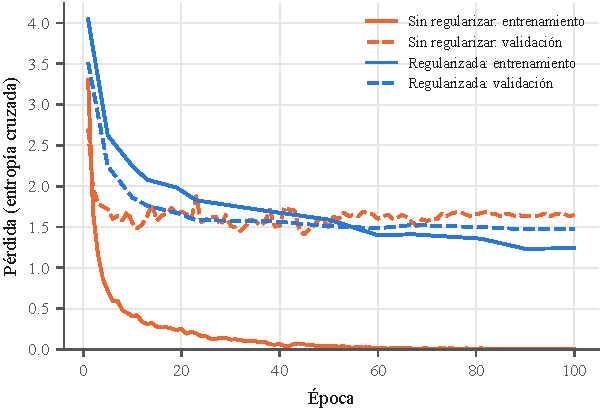
\includegraphics[width=0.75\textwidth]{fig_sobreajuste}
  \caption{Pérdida de entrenamiento y de validación de la CNN de audio sin
  regularización y con la regularización completa. Sin regularización la red
  memoriza el conjunto de entrenamiento y la pérdida de validación deja de
  bajar; con regularización ambas curvas se mantienen cercanas.}
  \label{fig:sobreajuste}
\end{figure}}{}

\begin{figure}[!htb]
  \centering
  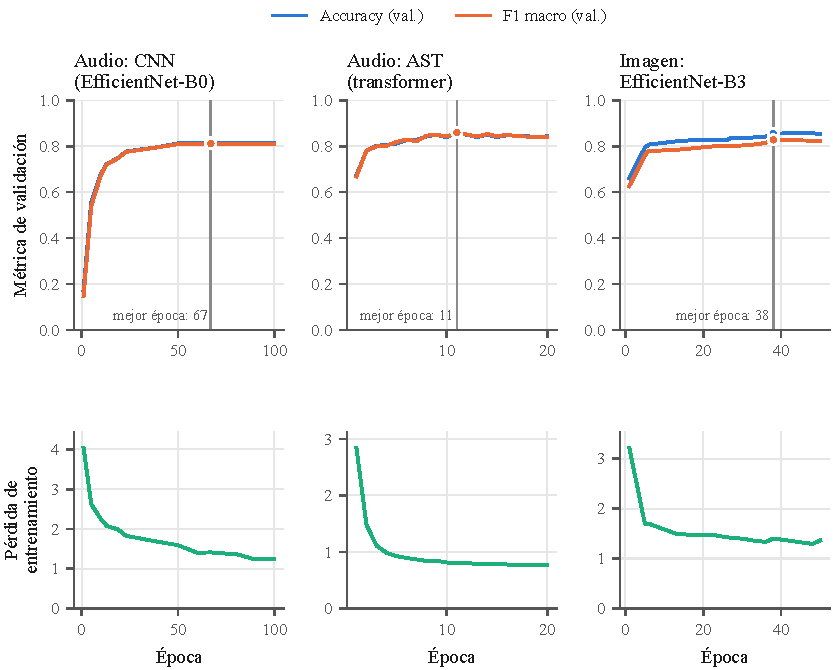
\includegraphics[width=\textwidth]{fig_curvas_entrenamiento}
  \caption{Curvas de entrenamiento de los tres clasificadores unimodales del sistema (CNN y AST de audio, EfficientNet-B3 de imagen): \textit{accuracy} y F1 macro en validación (arriba) y pérdida de
  entrenamiento (abajo). La línea vertical marca la época del mejor
  \textit{checkpoint}, que es el evaluado en prueba.}
  \label{fig:curvas}
\end{figure}

\subsection{Desempeño global}

La \tabref{tab:audio} y la \figref{fig:audio-cnn-ast} resumen el desempeño
en el conjunto de prueba (393 grabaciones, 55 especies). Ambos modelos
superan la meta de \SI{85}{\percent} de \textit{accuracy} con el protocolo
agregado y el AST supera a la CNN en los dos protocolos, con una diferencia
de dos puntos por ventana que se reduce a uno al agregar. La agregación por
grabación aporta entre 3,8 y 5,4 puntos sin reentrenar nada, porque promedia
ventanas sin vocalización o con ruido con las que sí contienen al ave focal.
Es la mitigación más barata del ruido de etiqueta de Xeno-canto descrito en
el \capref{cap:relacionado}. El costo del AST es alto: 86 millones de
parámetros frente a 4 millones, y 480 segundos por época frente a 22, es
decir, unas 20 veces más cómputo para un punto adicional de
\textit{accuracy}.

\begin{table}[!htb]
  \centering\small
  \caption{Clasificadores de audio en el conjunto de prueba (393 grabaciones,
  55 especies). El protocolo agregado promedia las probabilidades de hasta 12
  ventanas (CNN) u 8 (AST) de la grabación.}
  \label{tab:audio}
  \setlength{\tabcolsep}{4pt}\footnotesize
  \begin{tabular}{@{}l r r r r r r@{}}
    \toprule
    & \multicolumn{2}{c}{Ventana única} & \multicolumn{2}{c}{Agregado} & & \\
    \cmidrule(lr){2-3}\cmidrule(lr){4-5}
    Modelo & \textit{Accuracy} & F1 macro & \textit{Accuracy} & F1 macro & Parámetros & Tiempo/época \\
    \midrule
    EfficientNet-B0 sin regularizar & 0,735 & 0,736 & 0,789 & 0,784 & 4,1 M & \SI{22}{\second} \\
    EfficientNet-B0 regularizada & 0,812 & 0,811 & \textbf{0,858} & \textbf{0,858} & 4,1 M & \SI{22}{\second} \\
    AST (AudioSet) & 0,832 & 0,828 & \textbf{0,870} & \textbf{0,864} & 86,2 M & \SI{480}{\second} \\
    \bottomrule
  \end{tabular}
\end{table}

\begin{figure}[!htb]
  \centering
  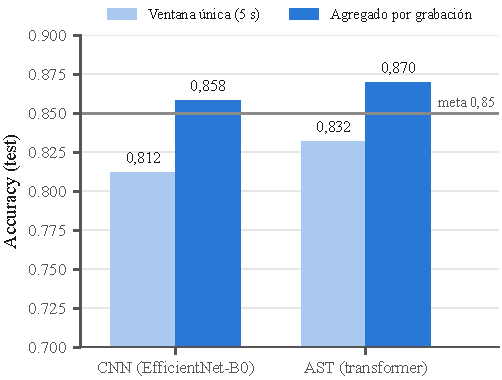
\includegraphics[width=0.6\textwidth]{fig_audio_cnn_vs_ast}
  \caption{\textit{Accuracy} en prueba de los clasificadores de audio con
  ventana única y con agregación por grabación.}
  \label{fig:audio-cnn-ast}
\end{figure}

La \tabref{tab:eval-extended} completa la caracterización con las métricas
que no dependen de un umbral de decisión. El AUC-ROC macro supera 0,99 en
los tres clasificadores del sistema y la especie correcta está entre las cinco más
probables en el \SI{97}{\percent} de las grabaciones (CNN) y el
\SI{95}{\percent} de las fotografías, lo que importa para un uso asistido en
que el sistema propone candidatas a un observador. La latencia mediana por
grabación, incluido el cálculo del espectrograma, es de \SI{18}{\milli\second}
para la CNN y \SI{177}{\milli\second} para el AST en la GPU del equipo. Una
fotografía con TTA tarda \SI{66}{\milli\second} (\SI{11}{\milli\second} con un
solo recorte).

\begin{table}[!htb]
  \centering\small
  \caption{Métricas extendidas de los clasificadores unimodales (solo audio o solo imagen) en el conjunto de prueba (protocolo operacional). AUC-ROC macro (cada especie frente a las demás); top-5: la especie correcta está entre las cinco más probables; latencia mediana por muestra en Apple M4 Pro (MPS), incluido el cálculo de características.}
  \label{tab:eval-extended}
  \footnotesize\setlength{\tabcolsep}{4pt}
  \begin{tabular}{@{}l r r r r r r@{}}
    \toprule
    Modelo & \textit{Accuracy} & F1 macro & AUC macro & Top-5 & Parámetros & Latencia (ms) \\
    \midrule
    Audio: CNN (agregado) & 0,858 & 0,858 & 0,991 & 0,969 & 4,1 M & 18 \\
    Audio: AST (agregado) & 0,870 & 0,864 & 0,993 & 0,949 & 86,2 M & 177 \\
    Imagen: B3 (TTA) & 0,848 & 0,808 & 0,990 & 0,948 & 10,8 M & 66 \\
    \bottomrule
  \end{tabular}
\end{table}


\textbf{Origen de la grabación.} Como el \SI{36}{\percent} del corpus
proviene de otros países, se evaluó por separado el desempeño sobre las 255
grabaciones chilenas y las 138 extranjeras del conjunto de prueba. La CNN
obtiene 0,847 de \textit{accuracy} en las chilenas y 0,877 en las
extranjeras (F1 macro 0,847 y 0,797). El AST obtiene 0,871 y 0,870. No hay,
por tanto, una penalización sobre las grabaciones chilenas: el desplazamiento de
dominio que se anticipó en el \capref{cap:datos} no se manifiesta en el
conjunto de prueba, en parte porque las grabaciones extranjeras pertenecen a
las mismas especies y a poblaciones vecinas (Argentina aporta la mitad de
ellas) y en parte porque el modelo aprende rasgos del canto más que del
ambiente de grabación.

\subsection{Desempeño por especie y por grupo de conservación}

La \figref{fig:f1-especie} (panel izquierdo) muestra el F1 de la CNN por
especie. Veintiséis especies superan 0,9 y solo ocho quedan bajo 0,7. La
\figref{fig:confusion} muestra en qué se equivoca el modelo y revela un
patrón distinto del esperado: los errores de audio \emph{no} se concentran
en pares de congéneres. De los 56 errores de la CNN en las 393 grabaciones,
solo tres ocurren entre especies del mismo género (\textit{Phrygilus gayi}
clasificado como \textit{P.~patagonicus}) y el resto se reparte en más de
cuarenta pares distintos, casi todos con un único caso. Las especies de peor
F1 (\textit{Cinclodes patagonicus} con 0,46, y \textit{Leptasthenura
aegithaloides}, \textit{Sylviorthorhynchus desmurii} y \textit{P.~gayi} con
0,62) fallan hacia una especie diferente en cada grabación, un patrón más
compatible con el ruido de etiqueta de Xeno-canto (especies de fondo, tramos
sin vocalización, llamados poco característicos) que con una similitud
acústica sistemática. El AST comete 51 errores con la misma dispersión. El
segundo factor es el \emph{tamaño del conjunto de prueba}: \textit{Agriornis
albicauda} (0,50) tiene tres grabaciones de prueba, de modo que un solo error
cuesta 33 puntos de \textit{recall}. La variabilidad de BirdNET entre
especies y contextos \citep{perezgranados2023birdnet} tiene aquí su
contraparte: el desempeño por especie depende tanto de la calidad de las
grabaciones disponibles como de la especie misma.

\begin{figure}[!htb]
  \centering
  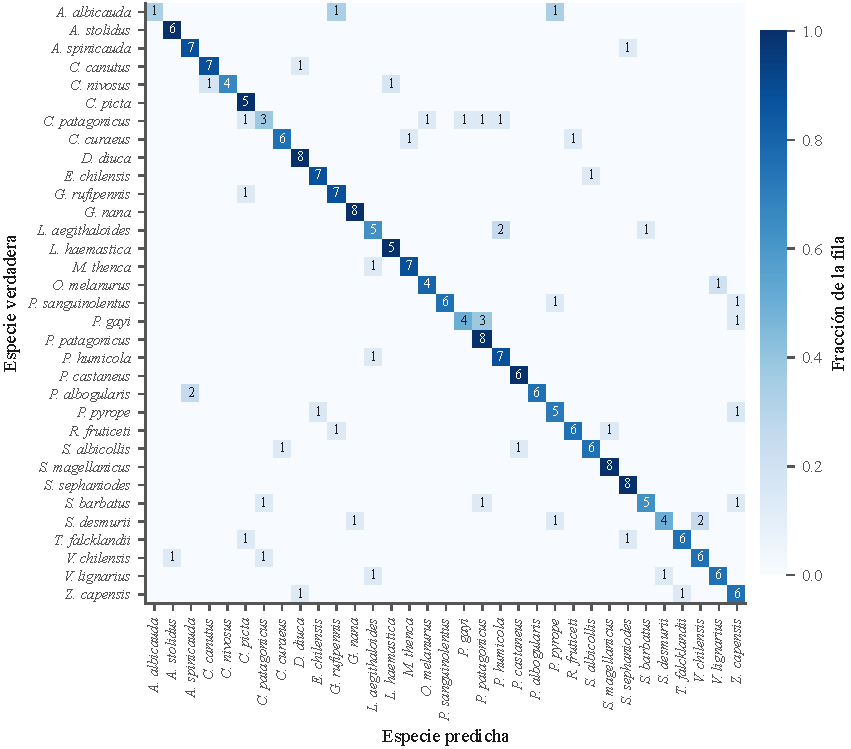
\includegraphics[width=0.9\textwidth]{fig_confusion_audio}
  \caption{Matriz de confusión de la CNN de audio (conjunto de prueba,
  agregado por grabación) restringida a las especies con \textit{recall}
  inferior a 0,8 y a las especies con que se confunden; el color indica la
  fracción de la fila y el número, las grabaciones. Los errores están
  dispersos: ningún par de especies acumula más de tres casos.}
  \label{fig:confusion}
\end{figure}

\begin{figure}[!htb]
  \centering
  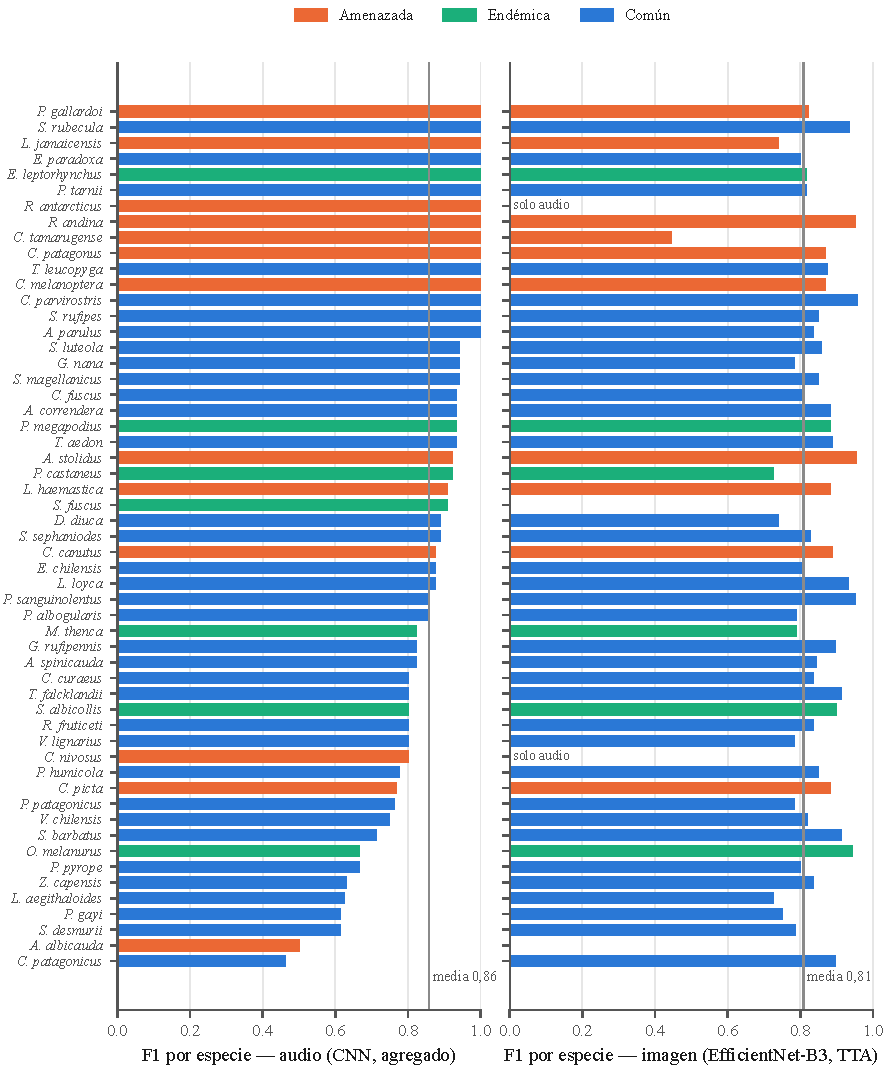
\includegraphics[width=\textwidth]{fig_f1_por_especie}
  \caption{F1 por especie en el conjunto de prueba del clasificador de audio
  (CNN, agregado por grabación) y del clasificador de imagen (EfficientNet-B3
  con TTA), coloreado por grupo de conservación y ordenado por el F1 de
  audio. Las dos especies sin fotografías suficientes no participan del
  clasificador de imagen.}
  \label{fig:f1-especie}
\end{figure}

Contra lo que la escasez de datos haría esperar, las especies amenazadas
obtienen en audio un F1 medio \emph{mayor} que las comunes, 0,906 frente a
0,838 (\tabref{tab:por-grupo}). Dos factores lo explican. Las amenazadas del conjunto son en su mayoría aves acuáticas, playeros y
loros, con vocalizaciones muy distintas de las de los paseriformes (el orden
de las aves cantoras, al que pertenece la mayoría de las especies pequeñas
del corpus), de modo que el problema \textit{fine-grained} es más fácil para
ellas. Además, sus conjuntos de prueba son pequeños, lo que hace sus métricas más altas pero también más inciertas. Las comunes, en cambio, concentran las especies de canto más variable y
las grabaciones más heterogéneas. El AST reparte el desempeño de forma más
pareja (F1 0,866, 0,896 y 0,857 en amenazadas, endémicas y comunes) y es el
mejor modelo en las endémicas. El desafío de la escasez de datos se
manifiesta, por tanto, menos en la métrica de prueba de las amenazadas que
en su variabilidad y en la dependencia de grabaciones extranjeras.

\begin{table}[!htb]
  \centering\small
  \caption{Desempeño por grupo de conservación. F1 medio por especie en el conjunto de prueba (audio: CNN, agregado por grabación; imagen: EfficientNet-B3 con TTA; fusión: pareo por especie) y AUC-ROC medio del SDM.}
  \label{tab:por-grupo}
  \fitwidth{\begin{tabular}{@{}l r r r r r r r@{}}
    \toprule
    Grupo & Especies & F1 audio & Especies & F1 imagen & F1 fusión & AUC MaxEnt & AUC RF \\
    \midrule
    Amenazada & 13 & 0,906 & 11 & 0,756 & 0,945 & 0,948 & 0,967 \\
    Endémica & 7 & 0,865 & 7 & 0,723 & 0,940 & 0,899 & 0,917 \\
    Común & 35 & 0,838 & 35 & 0,842 & 0,942 & 0,827 & 0,849 \\
    \midrule
    Todas & 55 & 0,858 & 53 & 0,808 & 0,942 & 0,863 & 0,884 \\
    \bottomrule
  \end{tabular}}
\end{table}


%-----------------------------------------------------------------------
\section{Identificación por imagen}\label{sec:res-imagen}

Se ajustó EfficientNet-B3 preentrenada en ImageNet, con entrada de
\SI{384}{px}, durante 50 épocas con la misma receta de regularización
(\textit{mixup}, suavizado de etiquetas, \textit{dropout}, profundidad
estocástica) y aumentación geométrica y de color. Una variante con pesos
NoisyStudent no mejoró la \textit{accuracy} (0,845 frente a 0,848), aunque sí
el F1 macro (0,820 frente a 0,808); se mantuvo la de ImageNet como rama del
sistema por su mejor \textit{accuracy} y porque la diferencia queda dentro del
intervalo de confianza. Una arquitectura mayor
(ConvNeXt preentrenada en ImageNet-21k) se descartó porque cada época tardaba
unas ocho horas en el equipo disponible, y ViT-B a \SI{384}{px}, comparable
a ConvNeXt, era inviable por el mismo motivo. Sí se entrenó la variante
pequeña de la familia, ViT-S/16 (21,7 M de parámetros, un cuarto de ViT-B;
preentrenado en ImageNet-21k y ajustado en ImageNet-1k), a \SI{224}{px}
durante 30 épocas (unos \SI{100}{\second} por época) con la misma receta de
regularización. Alcanzó 0,797 de \textit{accuracy} en validación, todavía
subiendo levemente al final, y 0,779 en prueba con recorte central (F1 macro
0,750), seis puntos por debajo de EfficientNet-B3 con el mismo protocolo
(0,839) y ocho con TTA, que al ViT lo empeora (0,767), posiblemente porque
sin la equivariancia de la convolución es más sensible al desplazamiento de
los recortes de esquina. El resultado es compatible con lo esperado para un
modelo con menos sesgos inductivos ajustado con unos pocos miles de
fotografías (\secref{sec:teoria-transformers}), pero la comparación está
confundida por la resolución (224 frente a \SI{384}{px}) y el número de
épocas, de modo que no permite concluir que la atención global no ayude
(\secref{sec:limitaciones}). A esta escala y con este cómputo, B3 sigue
siendo la rama de imagen del sistema. La \tabref{tab:imagen} resume los
resultados en las \num{1040} fotografías de prueba (53 especies).

\begin{table}[!htb]
  \centering\small
  \caption{Clasificadores de imagen en el conjunto de prueba (\num{1040}
  fotografías, 53 especies).}
  \label{tab:imagen}
  \begin{tabular}{@{}l r r r r r@{}}
    \toprule
    & \multicolumn{2}{c}{Recorte central} & \multicolumn{2}{c}{TTA (10 vistas)} & \\
    \cmidrule(lr){2-3}\cmidrule(lr){4-5}
    Modelo & \textit{Accuracy} & F1 macro & \textit{Accuracy} & F1 macro & Parámetros \\
    \midrule
    EfficientNet-B3 (ImageNet) & 0,839 & 0,802 & \textbf{0,848} & 0,808 & 10,8 M \\
    EfficientNet-B3 (NoisyStudent) & -- & -- & 0,845 & 0,820 & 10,8 M \\
    ViT-S/16 (ImageNet-21k, \SI{224}{px}) & 0,779 & 0,750 & 0,767 & 0,727 & 21,7 M \\
    \bottomrule
  \end{tabular}
\end{table}

El clasificador de imagen queda dos milésimas bajo la meta de 0,85 cuando se
evalúa solo. La curva de validación (\figref{fig:curvas}) muestra un
\textit{plateau} desde la época 36, de modo que más épocas no ayudan, y el
techo está en las especies difíciles: en el panel derecho de la
\figref{fig:f1-especie}, \textit{Scytalopus fuscus} (F1 0,00, cinco
fotografías de prueba) es visualmente casi idéntico a su congénere
\textit{S.~magellanicus}, y \textit{Agriornis albicauda} (0,00, dos
fotografías) y \textit{Conirostrum tamarugense} (0,44, tres) son las especies
con menos ejemplos. Diez especies superan 0,9. A diferencia del audio, en
imagen los errores sí se concentran en congéneres: el \SI{13}{\percent} de los
158 errores ocurre dentro de un género, y los pares más frecuentes son
\textit{Phrygilus gayi} y \textit{P.~patagonicus} (nueve casos en ambos
sentidos), los dos \textit{Scytalopus}, \textit{Pteroptochos castaneus} y
\textit{P.~tarnii}, y los dos \textit{Chloephaga}. También a diferencia del
audio, aquí las amenazadas y endémicas rinden peor que las comunes, con F1
medio de 0,756 y 0,723 frente a 0,842 (\tabref{tab:por-grupo}): en imagen la
escasez de
ejemplos pesa más que la distintividad, porque un plumaje se parece a otro
más de lo que un canto se parece a otro. Dado que la meta de
\SI{85}{\percent} se definió para el sistema multimodal, se aceptó este
resultado como la rama visual del sistema. La sección siguiente muestra que
la fusión la supera con amplitud.

%-----------------------------------------------------------------------
\section{Fusión multimodal}\label{sec:res-fusion}

\subsection{\textit{Late fusion} frente a cada modalidad}

La \textit{late fusion} combina las probabilidades de la CNN de audio (55 clases,
agregadas por grabación) y de EfficientNet-B3 (53 clases, proyectadas al
espacio de 55 con probabilidad cero para las dos especies que solo tienen audio) con
peso $\alpha = 0{,}5$ (Ecuación~\ref{eq:fusion}). Siguiendo el protocolo del
\capref{cap:teoria}, el pareo por especie se repitió 20 veces con semillas
distintas (30 pares por especie, \num{1590} pares por repetición, 53
especies) y se reportan la media y la desviación estándar
(\tabref{tab:fusion-summary}, \figref{fig:fusion}). Con la CNN como rama
de audio, la fusión alcanza \textbf{0,945 $\pm$ 0,004} de \textit{accuracy} y
0,942 $\pm$ 0,004 de F1 macro, frente a 0,865 $\pm$ 0,008 del audio solo y
0,816 $\pm$ 0,009 de la imagen sola sobre los mismos pares: 8,0 puntos sobre
la mejor modalidad y 12,9 sobre la imagen, con una variabilidad entre
repeticiones diez veces menor que la ganancia (el pareo único usado durante
el desarrollo había dado 0,950, dentro del rango). La meta del
\SI{85}{\percent} se supera con holgura y se confirma la hipótesis central
del Módulo 1.

\begin{table}[!htb]
  \centering\small
  \caption{\textit{Late fusion} evaluada con pareo por especie repetido: media y desviación estándar sobre 20 repeticiones de 1590 pares (53 especies), para las dos ramas de audio disponibles.}
  \label{tab:fusion-summary}
  \footnotesize
  \begin{tabular}{@{}l l r r@{}}
    \toprule
    Rama de audio & Modalidad & \textit{Accuracy} & F1 macro \\
    \midrule
    CNN (EfficientNet-B0) & Audio solo & 0,865 $\pm$ 0,008 & 0,861 $\pm$ 0,009 \\
    CNN (EfficientNet-B0) & Imagen sola & 0,816 $\pm$ 0,009 & 0,803 $\pm$ 0,009 \\
    CNN (EfficientNet-B0) & \textit{Late fusion} ($\alpha=0{,}5$) & 0,945 $\pm$ 0,004 & 0,942 $\pm$ 0,004 \\
    CNN (EfficientNet-B0) & Mejor fusión ($\alpha=0{,}5$, geométrica) & 0,956 $\pm$ 0,004 & 0,954 $\pm$ 0,004 \\
    AST & Audio solo & 0,877 $\pm$ 0,010 & 0,872 $\pm$ 0,010 \\
    AST & Imagen sola & 0,816 $\pm$ 0,009 & 0,803 $\pm$ 0,009 \\
    AST & \textit{Late fusion} ($\alpha=0{,}5$) & 0,946 $\pm$ 0,006 & 0,941 $\pm$ 0,006 \\
    AST & Mejor fusión ($\alpha=0{,}5$, geométrica) & 0,953 $\pm$ 0,005 & 0,948 $\pm$ 0,005 \\
    \bottomrule
  \end{tabular}
\end{table}


\begin{figure}[!htb]
  \centering
  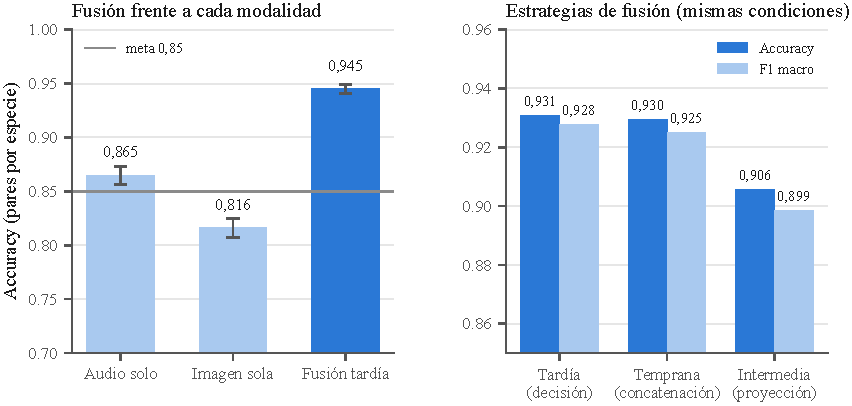
\includegraphics[width=\textwidth]{fig_fusion}
  \caption{Fusión multimodal evaluada con pareo por especie (\num{1590}
  pares, 53 especies). Izquierda: la \textit{late fusion} frente a cada modalidad
  sobre los mismos pares (media de 20 repeticiones; las barras de error,
  apenas visibles, son la desviación estándar). Derecha: comparación
  controlada de tres estrategias de fusión con cabezas entrenadas sobre los
  \textit{frozen embeddings} de ambos modelos.}
  \label{fig:fusion}
\end{figure}

El análisis de complementariedad explica la ganancia. En el
\SI{71,6}{\percent} de los pares ambas modalidades aciertan, en el
\SI{14,9}{\percent} solo el audio, en el \SI{10,0}{\percent} solo la imagen y
en el \SI{3,5}{\percent} ninguna. La fusión resuelve correctamente el
\SI{91,6}{\percent} de los pares en que las modalidades discrepan y no
estropea ninguno en que ambas aciertan: su techo, si resolviera todas las
discrepancias, sería 0,965, y alcanza 0,945. Cuando el audio confunde dos
\textit{Phrygilus}, la fotografía los separa. Cuando la imagen no distingue
dos \textit{Scytalopus}, el canto sí lo hace. El efecto es más visible por
grupo de conservación (\tabref{tab:por-grupo}): la fusión lleva a las
especies endémicas, las peores en imagen (F1 0,723) y medianas en audio
(0,865), a 0,940, y deja a los tres grupos entre 0,94 y 0,95. Con ello borra
la desventaja de las especies con menos datos.

\begin{figure}[!htb]
  \centering
  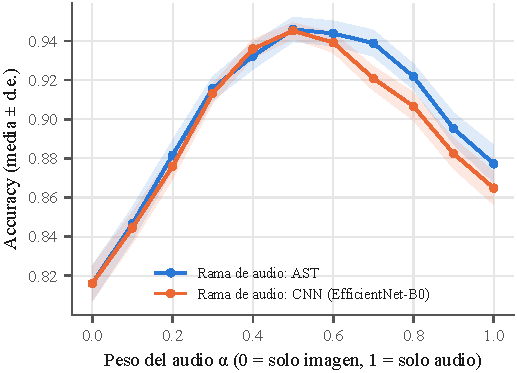
\includegraphics[width=0.6\textwidth]{fig_fusion_alpha}
  \caption{Sensibilidad de la \textit{late fusion} al peso del audio $\alpha$
  (media aritmética de probabilidades), con la CNN o el AST como rama de
  audio; banda: desviación estándar sobre 20 repeticiones del pareo.}
  \label{fig:fusion-alpha}
\end{figure}

La \figref{fig:fusion-alpha} muestra la sensibilidad al peso $\alpha$. La
curva es unimodal con máximo en $\alpha = 0{,}5$ y una meseta entre 0,4 y
0,6, y es asimétrica a favor del audio: con $\alpha = 0{,}7$ la fusión
todavía supera 0,92, mientras que con $\alpha = 0{,}3$ cae a 0,91. La media
geométrica de probabilidades (producto de expertos) mejora un punto sobre la
aritmética (0,956 $\pm$ 0,004) porque penaliza las clases que una modalidad
descarta con seguridad. Reemplazar la CNN por el AST en la rama de audio,
pese a sus 1,2 puntos adicionales en solitario (0,877 $\pm$ 0,010), no cambia
la fusión (0,946 $\pm$ 0,006): la ganancia proviene de la complementariedad,
no de la fuerza de cada rama. En síntesis, el sistema final usa la CNN como
rama de audio y \textit{late fusion} con $\alpha = 0{,}5$, que alcanza
0,945 $\pm$ 0,004 de \textit{accuracy} (intervalo de confianza al
\SI{95}{\percent} de 0,924 a 0,959). La variante con media geométrica es la
de mayor precisión observada (0,956 $\pm$ 0,004, con intervalo de 0,937 a
0,972). El sistema conserva la media aritmética por dos razones: los
intervalos de confianza de ambas variantes se solapan, y la media geométrica
anula cualquier especie a la que una rama asigne probabilidad cero, lo que
ocurre con las dos especies que solo tienen audio cuando la rama de imagen se
proyecta de 53 a 55 clases. La
diferencia entre usar la CNN o el AST como rama de audio (0,001) es menor
que una desviación estándar, de modo que no justifica un modelo veinte veces
más costoso.

\subsection{Comparación de estrategias de fusión}

Para aislar el efecto de la arquitectura de fusión se compararon las tres
estrategias de la taxonomía de \citet{baltrusaitis2019multimodal} en
condiciones idénticas: los mismos \textit{backbones} ya entrenados,
congelados como extractores de características (1\,280 dimensiones de audio y
1\,536 de imagen), los mismos pares por especie (150 de entrenamiento y 30 de
prueba por especie) y cabezas con la misma configuración (40 épocas, tasa de
aprendizaje $10^{-3}$, lotes de 64). La \textit{late fusion} entrena una cabeza
lineal por modalidad y promedia sus probabilidades. La \textit{early fusion}
concatena los dos \textit{embeddings} a la entrada de una única cabeza, y la
\textit{intermediate fusion} proyecta cada modalidad a un espacio común de 256
dimensiones antes de concatenar. El panel derecho de la \figref{fig:fusion}
muestra el resultado: la \textit{late fusion} (0,931) y la
\textit{early fusion} (0,930) empatan y la \textit{intermediate fusion} queda
por debajo
(0,906). Las proyecciones por modalidad agregan parámetros que sobreajustan
con los pares disponibles, y como los \textit{embeddings} ya son
representaciones de alto nivel, la transformación adicional no aporta. El
resultado respalda la elección de la \textit{late fusion} para el sistema final,
que además es robusta a modalidades faltantes. (El 0,945 de la subsección
anterior promedia los \textit{softmax} de los modelos completos, sin cabeza
adicional, por lo que es algo superior a las cabezas entrenadas sobre
\textit{frozen embeddings}.)

%-----------------------------------------------------------------------
\section{\textit{Baselines} de referencia}\label{sec:res-baselines}

Dos referencias sitúan el aporte de los modelos ajustados. La primera es la
de ``bajo costo'': un clasificador lineal sobre los \textit{frozen embeddings} de un modelo preentrenado, siguiendo el protocolo de
\citet{ghani2023embeddings}, con regresión logística multinomial y el
parámetro de regularización elegido en validación. Se usaron tres
extractores sin ajustar: EfficientNet-B0 de ImageNet sobre el espectrograma
log-mel, el AST de AudioSet (salida de 768 dimensiones) y EfficientNet-B3 de
ImageNet sobre la fotografía. La segunda referencia es un \emph{modelo de IA
generativa multimodal} (Claude, Anthropic;
\citealp{anthropic2026claude}) consultado mediante la API con cada
fotografía del conjunto de prueba y la lista cerrada de las 53 especies
candidatas, en modo \textit{zero-shot} (solo la lista) y \textit{few-shot}
(una fotografía de referencia por especie, tomada del conjunto de
entrenamiento). La respuesta se restringe a un nombre de la lista mediante
salida estructurada, de modo que el protocolo de métricas es el mismo del
clasificador propio.

\begin{table}[!htb]
  \centering\small
  \caption{\textit{Baselines} de referencia frente a los modelos ajustados (conjuntos de prueba). \textit{Frozen embeddings}: regresión logística sobre las representaciones de un modelo preentrenado sin ajustar. IA generativa: modelo de IA generativa multimodal consultado con la fotografía y la lista cerrada de especies.}
  \label{tab:baselines}
  \footnotesize
  \begin{tabularx}{\textwidth}{@{}l >{\raggedright\arraybackslash}X r r r@{}}
    \toprule
    Modalidad & Método & \textit{Accuracy} & F1 macro & AUC macro \\
    \midrule
    Audio & \textit{Frozen embeddings} de EfficientNet-B0 (ImageNet) + regresión logística & 0,547 & 0,545 & 0,901 \\
    Audio & \textit{Frozen embeddings} de AST (AudioSet) + regresión logística & 0,784 & 0,769 & 0,980 \\
    Imagen & \textit{Frozen embeddings} de EfficientNet-B3 (ImageNet) + regresión logística & 0,775 & 0,760 & 0,985 \\
    Imagen & IA generativa (claude-opus-5-5, \textit{zero-shot}, esfuerzo \textit{low}) & 0,803 & 0,765 & -- \\
    Imagen & IA generativa (claude-opus-5-5, \textit{few-shot}, esfuerzo \textit{low}) & 0,817 & 0,779 & -- \\
    \midrule
    Audio & \textbf{CNN EfficientNet-B0 ajustada (este trabajo)} & 0,858 & 0,858 & 0,991 \\
    Audio & \textbf{AST ajustado (este trabajo)} & 0,870 & 0,864 & 0,993 \\
    Imagen & \textbf{EfficientNet-B3 ajustada + TTA (este trabajo)} & 0,848 & 0,808 & 0,990 \\
    \bottomrule
  \end{tabularx}
\end{table}


\textbf{\textit{Frozen embeddings}.} Sobre el espectrograma, las características
de EfficientNet-B0 preentrenada en ImageNet, sin ajuste, llegan solo a
0,547 de \textit{accuracy} (\tabref{tab:baselines}): las representaciones
de imágenes naturales describen mal un espectrograma, y el ajuste completo
aporta 31 puntos. El AST preentrenado en AudioSet, un modelo de audio
general, transfiere mucho mejor (0,784 con una regresión logística) y el
ajuste agrega 8,6 puntos. El orden entre ambos extractores reproduce el
hallazgo de \citet{ghani2023embeddings} de que el preentrenamiento en el
dominio correcto importa más que la arquitectura. En imagen,
EfficientNet-B3 congelada da 0,775 y el ajuste suma 7,3 puntos. En las tres
ramas el AUC-ROC de la referencia congelada es alto (0,90 a 0,99): el
ordenamiento de candidatas es razonable sin ajustar, pero la decisión final
no lo es.

\textbf{IA generativa.} Claude Opus 5.5 identifica correctamente el
\SI{80,3}{\percent} de las \num{1040} fotografías de prueba en
\textit{zero-shot} (F1 macro 0,765), 4,5 puntos por debajo de
EfficientNet-B3 ajustada (0,848 de \textit{accuracy} y 0,808 de F1) y 14 por
debajo de la fusión multimodal. Cuatro fotografías fueron rechazadas por un
error de formato (archivos PNG con extensión JPEG, corregido en las corridas
posteriores) y cuentan como errores. La brecha entre su \textit{accuracy} y su F1 macro se explica por
cómo promedia cada métrica: la \textit{accuracy} cuenta aciertos sobre las
\num{1040} fotografías, donde pesan las especies comunes con 22 fotografías
de prueba, mientras que el F1 macro promedia el F1 de cada especie por
igual, de modo que las endémicas y las especies con dos o tres fotografías,
donde el modelo falla, pesan tanto como las comunes bien resueltas. El perfil por grupo es revelador: el modelo generativo
es excelente en las especies amenazadas (F1 0,839 y \SI{93}{\percent} de
acierto), que son aves acuáticas, playeros y loros abundantemente
fotografiados en todo el mundo, y competente en las comunes (0,795), pero
falla en las endémicas (F1 0,498 y \SI{56}{\percent} de acierto): confunde
sistemáticamente los tapaculos chilenos (turca 0,42, tapaculo 0,31, hued-hued
castaño 0,36, churrín del norte 0,25) y la chiricoca (0,40), especies que el
clasificador propio resuelve con F1 de 0,73 a 0,94. El modelo de IA generativa conoce las aves que el mundo fotografía y no las que solo Chile
tiene, que son justamente el foco de este trabajo. Supera al clasificador
especializado en 23 especies y pierde en 28. Su confianza declarada es
informativa (0,79 en los aciertos frente a 0,48 en los errores), lo que
permitiría abstenerse en los casos dudosos. El costo fue de US\$2,19 por el
conjunto completo (0,2 centavos por fotografía), con una latencia mediana de
\SI{2,4}{\second} por consulta frente a \SI{66}{\milli\second} del clasificador
propio en un equipo portátil.

En modo \textit{few-shot}, con una fotografía de referencia por especie
servida desde la caché de \textit{prompts}, el modelo sube a 0,817 de
\textit{accuracy} y 0,779 de F1 macro, sin respuestas inválidas. La mejora
se concentra donde faltaba conocimiento: las endémicas pasan de 0,498 a
0,567 de F1 (de \SI{56}{\percent} a \SI{71}{\percent} de acierto), con
ganancias de 14 a 27 puntos en la chiricoca, la turca y el tapaculo, mientras
que las amenazadas no cambian (0,837) y las comunes apenas (0,804). Una sola
fotografía de referencia cierra alrededor de un quinto de la brecha de las
endémicas respecto del clasificador propio, que sigue ganando en 29 especies
frente a 23, y el costo sube a US\$4,27 por el conjunto (0,4 centavos por
fotografía) con \SI{2,7}{\second} de latencia. La \figref{fig:llm-zero-few} resume el antes y el después por grupo. Ni en
\textit{zero-shot} ni en \textit{few-shot} el modelo generativo alcanza a la
rama de imagen ajustada con \num{4980} fotografías, y ambos quedan 13 puntos
por debajo de la fusión multimodal. La comparación responde el OE4 y, de
paso, justifica entrenar modelos propios para las especies que importan a la
conservación local.

\begin{figure}[!htb]
  \centering
  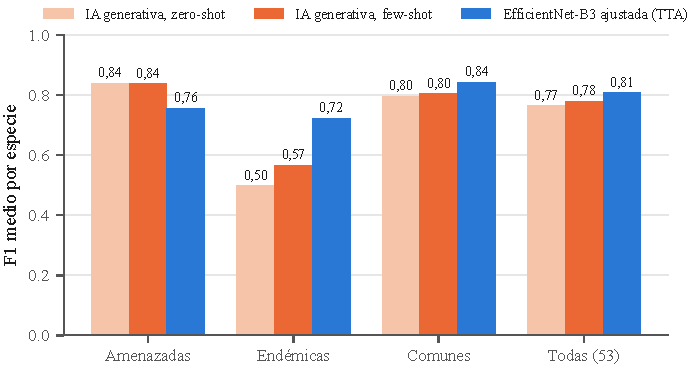
\includegraphics[width=0.8\textwidth]{fig_llm_zero_few}
  \caption{F1 medio por grupo de conservación del modelo generativo en
  \textit{zero-shot} y \textit{few-shot}, frente al clasificador de imagen
  ajustado. La fotografía de referencia mejora sobre todo a las endémicas, sin
  cerrar la brecha con el modelo propio.}
  \label{fig:llm-zero-few}
\end{figure}

%-----------------------------------------------------------------------
\section{Modelo de distribución espaciotemporal}\label{sec:res-sdm}

\subsection{Modelos comparados}

Sobre el conjunto de datos de la \secref{sec:datos-sdm} (presencias de cada
especie frente a \num{1500} puntos de fondo de grupo objetivo, muestreados
con la misma semilla para todos los modelos) se compararon cuatro
alternativas, cuyas bases se presentan en la \secref{sec:teoria-sdm}:
\begin{itemize}[leftmargin=*, itemsep=2pt]
  \item \textbf{MaxEnt} (\textit{baseline}): regresión logística penalizada
        con características lineales y cuadráticas y clases balanceadas,
        aprovechando la equivalencia entre MaxEnt y los modelos de regresión
        para datos de solo presencia \citep{fithian2013equivalence}.
  \item \textbf{Red neuronal conjunta}: el perceptrón multicapa multiespecie
        con dos capas ocultas de 64 unidades, \textit{dropout} de 0,3 y un
        \textit{embedding} de especie de 8 dimensiones, entrenado con entropía
        cruzada binaria ponderada durante 40 épocas sobre todas las especies a
        la vez.
  \item \textbf{Random Forest}: 300 árboles con clases balanceadas.
  \item \textbf{Gradient boosting}: 300 iteraciones con tasa de aprendizaje
        0,05 y clases balanceadas.
\end{itemize}
Todos usan las seis covariables (NDVI, temperatura, precipitación, elevación
y el mes cíclico) y se evalúan por especie con AUC-ROC sobre una partición
estratificada 70/30.

\begin{table}[!htb]
  \centering\small
  \caption{Modelos de distribución comparados: AUC-ROC medio sobre las 54 especies con al menos 20 presencias y número de especies en que cada modelo supera a MaxEnt. Partición aleatoria estratificada 70/30 y validación cruzada espacial por bloques de 200 km (5 \textit{folds}).}
  \label{tab:sdm-modelos}
  \footnotesize\setlength{\tabcolsep}{4pt}
  \fitwidth{\begin{tabular}{@{}l r r r r@{}}
    \toprule
    Modelo & AUC (aleatoria) & Gana a MaxEnt & AUC (espacial) & Gana a MaxEnt \\
    \midrule
    MaxEnt (regresión logística penalizada) & 0,863 & -- & 0,816 & -- \\
    Red neuronal conjunta & 0,856 & 15/54 & 0,810 & 21/54 \\
    Gradient boosting & 0,883 & 44/54 & 0,803 & 16/54 \\
    Random Forest & 0,884 & 46/54 & 0,812 & 17/54 \\
    \bottomrule
  \end{tabular}}
\end{table}


\begin{figure}[!htb]
  \centering
  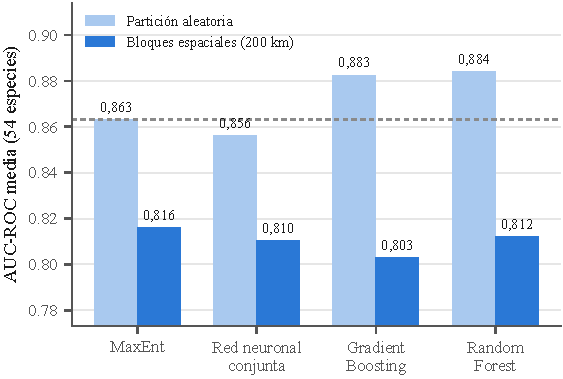
\includegraphics[width=0.62\textwidth]{fig_sdm_modelos}
  \caption{AUC-ROC medio de los modelos de distribución sobre las 54 especies
  modeladas. La línea punteada marca el \textit{baseline} MaxEnt.}
  \label{fig:sdm-modelos}
\end{figure}

El resultado (\tabref{tab:sdm-modelos}, \figref{fig:sdm-modelos}) contradice
la hipótesis original en su forma literal y la confirma en su espíritu. La
red neuronal \emph{no} supera a MaxEnt: obtiene 0,856 de AUC medio frente a
0,863 y solo gana en 15 de las 54 especies. Los ensambles de árboles, en
cambio, superan a MaxEnt con claridad: Random Forest alcanza 0,884 y gana en
46 de 54 especies, y gradient boosting 0,883 con 44 victorias. La mejora media de Random Forest sobre MaxEnt es de 0,021 (intervalo de
confianza al \SI{95}{\percent} de 0,015 a 0,027 y $p < 0{,}001$ en un test de
Wilcoxon pareado por especie), con casos de hasta siete puntos
(\textit{Vanellus chilensis} pasa de 0,725 a 0,795 y \textit{Limosa
haemastica} de 0,871 a 0,943) y ocho especies en que MaxEnt conserva una ventaja pequeña
(\figref{fig:sdm-especie}). La desventaja de la red neuronal también es
sistemática aunque pequeña (0,007 con $p = 0{,}001$). El patrón es coherente con la evidencia de que, en datos tabulares de
tamaño moderado, los modelos de árboles siguen superando a las redes
neuronales \citep{grinsztajn2022trees} y con los \textit{benchmarks} de SDM,
donde los árboles potenciados y los ensambles figuran entre los mejores
métodos.

\begin{figure}[!htb]
  \centering
  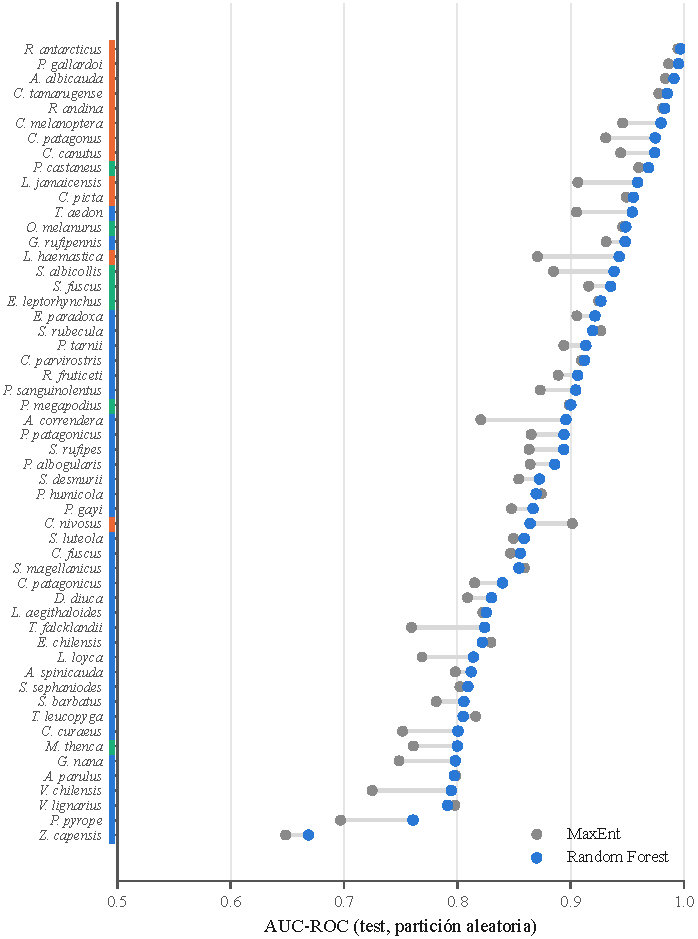
\includegraphics[width=0.78\textwidth]{fig_sdm_auc_especie}
  \caption{AUC-ROC por especie de MaxEnt y Random Forest (partición
  aleatoria), ordenadas por el valor de Random Forest; la franja de color
  indica el grupo de conservación.}
  \label{fig:sdm-especie}
\end{figure}

El desempeño por especie depende sobre todo de la amplitud de su
distribución. Las especies de rango restringido se modelan casi
perfectamente (\textit{Rallus antarcticus} 0,997, \textit{Podiceps gallardoi}
0,995, \textit{Agriornis albicauda} 0,991), mientras que los generalistas
ubicuos son los más difíciles (\textit{Zonotrichia capensis} 0,669,
\textit{Pyrope pyrope} 0,761): cuando una especie está en todas partes, el
fondo de grupo objetivo se parece a sus presencias y las covariables no
pueden separarlos. Por eso, al contrario del clasificador de imagen, aquí las
especies amenazadas obtienen el AUC más alto, 0,967 con Random Forest frente
a 0,849 de las comunes (\tabref{tab:por-grupo}): la escasez de registros no
impide modelarlas, porque sus pocos registros son ambientalmente muy
informativos.

\subsection{¿Aportan los datos satelitales no estructurados?}

Para dar al aprendizaje profundo una ventaja que MaxEnt no puede aprovechar,
se probaron dos fuentes de información satelital no estructurada
(\figref{fig:sdm-satelite}, panel izquierdo). Con parches de cobertura de
suelo de \SI{3}{\kilo\metre} procesados por una CNN junto a las covariables,
la red cayó a 0,613 de AUC, y con el \textit{embedding} satelital de 64
dimensiones de AlphaEarth, a 0,767. Se verificó que los parches estaban
correctamente alineados, de modo que la degradación no es un error de datos
sino sobreajuste: la cobertura de suelo es redundante con el NDVI y la
elevación (bosque donde el NDVI es alto, suelo desnudo donde es bajo o la
altitud es alta) y la capacidad adicional de la red solo agrega varianza.
La prueba definitiva es que el \textit{embedding} también perjudica a los
árboles, que son robustos a características irrelevantes: Random Forest baja
de 0,884 a 0,878 (una caída pequeña pero consistente en 44 de 54 especies,
$p < 0{,}001$) y gradient boosting de 0,883 a 0,881.

\begin{figure}[!htb]
  \centering
  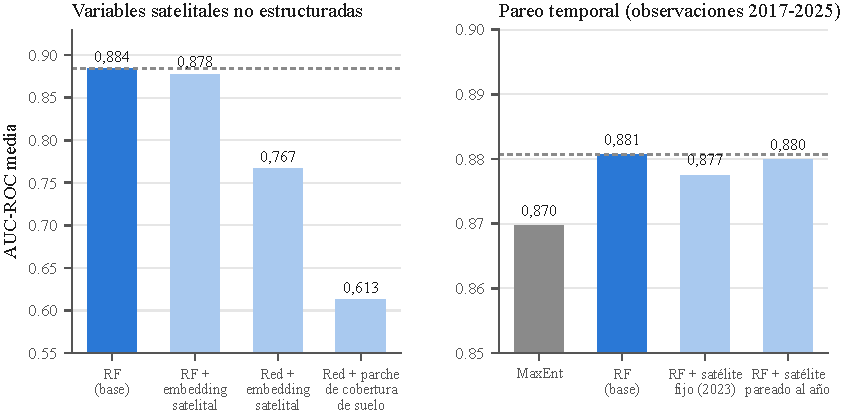
\includegraphics[width=\textwidth]{fig_sdm_satelite}
  \caption{Experimentos con información satelital. Izquierda: AUC-ROC medio
  al agregar el \textit{embedding} satelital o parches de cobertura de suelo
  a las covariables base. Derecha: pareo temporal del \textit{embedding}
  satelital al año de cada observación, sobre el subconjunto 2017--2025 (53
  especies).}
  \label{fig:sdm-satelite}
\end{figure}

Quedaba una explicación alternativa: el desajuste temporal entre la imagen
satelital (un compuesto fijo de 2023) y observaciones de cualquier año. Para
descartarla se repitió el experimento sobre las observaciones de 2017 a
2025, pareando a cada punto el NDVI y el \textit{embedding} del año en que
fue observado (panel derecho de la \figref{fig:sdm-satelite}). El pareo ayuda marginalmente respecto del compuesto fijo (0,880 frente a
0,877 y mejor en 32 de 53 especies, $p = 0{,}010$), lo que confirma que el
desajuste existía, pero ninguna versión supera a las covariables base sin
satélite (0,881): la diferencia entre el satélite pareado y la base es
$-0{,}001$ con un intervalo de confianza de $-0{,}005$ a $+0{,}003$ ($p =
0{,}89$), es decir, indistinguible de cero (\tabref{tab:tests-sdm}; el test
se hace sobre Random Forest, el mejor modelo del bloque). El
desajuste temporal era un factor menor. La causa es la redundancia.

\subsection{Validación espacial por bloques}

Para comprobar que la comparación anterior no está inflada por la
autocorrelación espacial, se repitió con validación cruzada por bloques,
siguiendo el protocolo de \texttt{blockCV} \citep{valavi2019blockcv}. Los
semivariogramas empíricos de las covariables dan rangos de autocorrelación
de \SI{650}{\kilo\metre} (NDVI, precipitación) a \SI{1200}{\kilo\metre}
(temperatura, elevación), consecuencia del gradiente latitudinal de Chile.
Bloques de ese tamaño dejarían entre cuatro y seis en todo el país,
de modo que se usaron bloques de \SI{200}{\kilo\metre} (46 bloques),
asignados al azar a cinco \textit{folds} equilibrados en número de
registros: de 10\,700 a 17\,400 filas por \textit{fold} del conjunto apilado
por especie (presencias más los 1\,500 puntos de fondo de cada especie, que
se repiten entre especies), equivalentes a entre unos 5\,800 y 8\,900 de los
34\,926 puntos distintos. Cada modelo se
entrena en cuatro \textit{folds} y se evalúa en el quinto, con los mismos
puntos y el mismo fondo que la partición aleatoria. En 13 especies de rango
restringido, cuyas presencias caen en pocos bloques, solo dos a cuatro
\textit{folds} tienen presencias suficientes para calcular el AUC.

El resultado (\tabref{tab:sdm-modelos}, \figref{fig:sdm-modelos}) cambia la
lectura. Todos los modelos caen entre cinco y ocho puntos al extrapolar a
bloques no vistos (MaxEnt de 0,863 a 0,816, Random Forest de 0,884 a 0,812,
gradient boosting a 0,803 y la red a 0,810) y las diferencias entre ellos
quedan dentro de la variabilidad entre \textit{folds} (desviación estándar
media de 0,06). Random Forest supera a MaxEnt en solo 17 de las 54 especies, la diferencia
media es de $-0{,}004$ con un intervalo de confianza que incluye el cero (de
$-0{,}013$ a $+0{,}004$, con $p = 0{,}06$) y en 21 especies es menor que 0,01.
Por grupo, los árboles conservan
ventaja en las especies amenazadas (0,901 frente a 0,883) y la pierden en
las comunes (0,779 frente a 0,788) y endémicas (0,823 frente a 0,845). La
ventaja de los ensambles de árboles es, por tanto, una ventaja de
\emph{interpolación}: con registros en todo el territorio aprovechan
interacciones locales entre covariables que MaxEnt no modela, pero al
predecir en zonas sin registros las funciones de respuesta suaves de MaxEnt
generalizan igual o mejor. Para la pregunta de investigación esto significa
que el aprendizaje automático supera a MaxEnt en el uso habitual de un SDM
(describir la distribución donde hay datos), pero no al extrapolar a
regiones sin muestreo, que es el escenario que la validación por bloques
simula y el más exigente. La \tabref{tab:tests-sdm} reúne todas las
comparaciones pareadas de este capítulo.

\begin{table}[!htb]
  \centering\footnotesize
  \caption{Comparaciones pareadas por especie entre modelos de distribución: diferencia media de AUC-ROC con intervalo \textit{bootstrap} al \SI{95}{\percent}, número de especies en que el primer modelo supera al segundo y valor $p$ del test de Wilcoxon de rangos con signo (bilateral).}
  \label{tab:tests-sdm}
  \begin{tabular}{@{}l l r r r r@{}}
    \toprule
    Protocolo & Comparación & $n$ & $\Delta$AUC [IC 95\,\%] & Gana & $p$ \\
    \midrule
    aleatoria & Random Forest vs. MaxEnt & 54 &  0,021 [0,015; 0,027] & 46/54 & $<$0,001 \\
    aleatoria & Gradient boosting vs. MaxEnt & 54 &  0,019 [0,012; 0,026] & 44/54 & $<$0,001 \\
    aleatoria & Red neuronal vs. MaxEnt & 54 & -0,007 [-0,011; -0,003] & 15/54 & 0,001 \\
    aleatoria & RF + \textit{embedding} satelital vs. RF & 54 & -0,006 [-0,009; -0,004] & 10/54 & $<$0,001 \\
    espacial & Random Forest vs. MaxEnt & 54 & -0,004 [-0,012; 0,004] & 17/54 & 0,060 \\
    espacial & Gradient boosting vs. MaxEnt & 54 & -0,013 [-0,022; -0,004] & 16/54 & 0,003 \\
    espacial & Red neuronal vs. MaxEnt & 54 & -0,006 [-0,012; 0,000] & 21/54 & 0,044 \\
    temporal 2017-2025 & RF vs. MaxEnt & 53 &  0,011 [0,005; 0,017] & 38/53 & $<$0,001 \\
    temporal 2017-2025 & RF + satélite fijo vs. RF & 53 & -0,003 [-0,007; 0,000] & 21/53 & 0,069 \\
    temporal 2017-2025 & RF + satélite pareado vs. RF & 53 & -0,001 [-0,005; 0,003] & 28/53 & 0,891 \\
    temporal 2017-2025 & RF + satélite pareado vs. fijo & 53 &  0,002 [0,001; 0,004] & 32/53 & 0,010 \\
    \bottomrule
  \end{tabular}
\end{table}


\subsection{Mapas de distribución estimada}

La \figref{fig:sdm-mapas} muestra la probabilidad de presencia estimada por
Random Forest sobre la grilla de \SI{0,1}{\degree} para tres especies de
distribución contrastante: el chucao, propio del bosque templado lluvioso
del sur; el tricahue (EN), confinado a los valles del centro-norte; y el
comesebo de los tamarugales (EN), restringido a la Pampa del Tamarugal. En
los tres casos el mapa reproduce el rango conocido y los avistamientos caen
en las zonas de alta probabilidad, sin que el modelo haya recibido las
coordenadas como covariable: la distribución emerge del clima, la vegetación
y la elevación. La \figref{fig:sdm-estacional} ilustra el eje temporal con el
zarapito de pico recto (VU), un playero migratorio que pasa el verano austral
en Chile: el modelo asigna alta probabilidad a los humedales del sur en enero
y la reduce en julio, cuando la especie está en el hemisferio norte, aunque
con la salvedad de que la mitad de los registros se concentra en verano por
el propio esfuerzo de observación.

\begin{figure}[!htb]
  \centering
  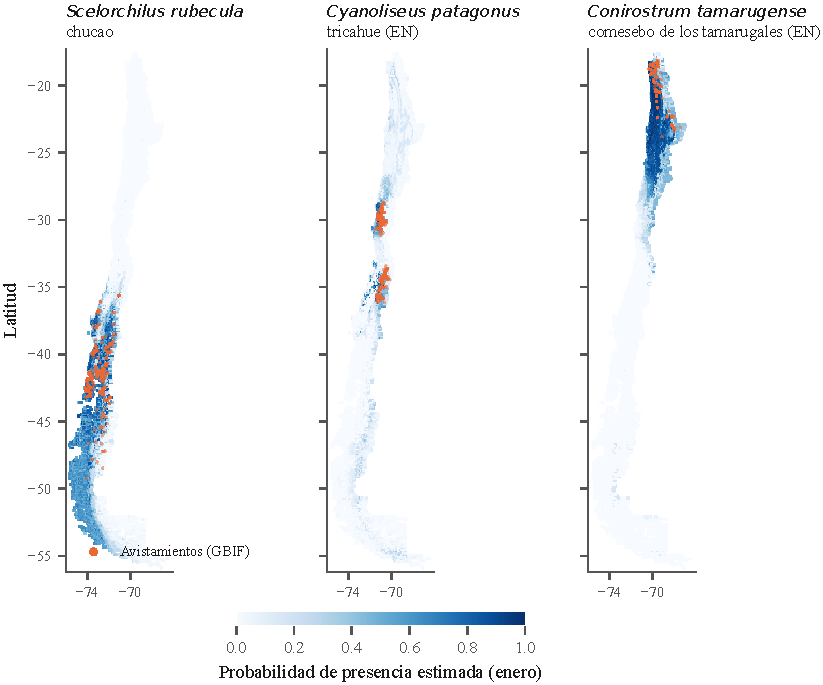
\includegraphics[width=\textwidth]{fig_sdm_mapas}
  \caption{Probabilidad de presencia en enero estimada por Random Forest para
  tres especies de distribución contrastante, con una muestra de sus
  avistamientos superpuesta.}
  \label{fig:sdm-mapas}
\end{figure}

\begin{figure}[!htb]
  \centering
  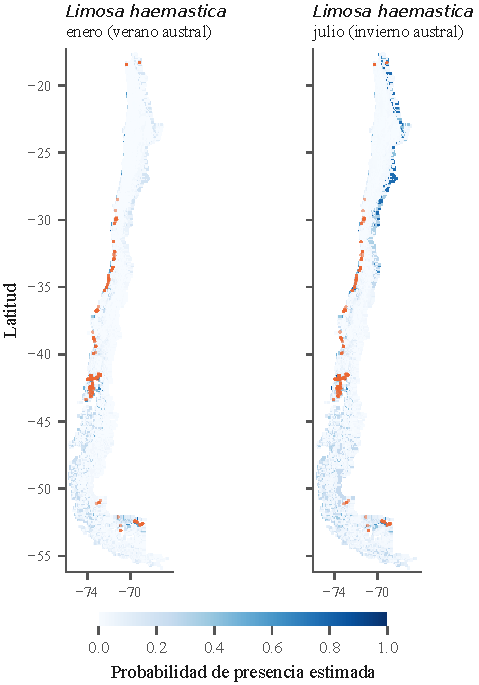
\includegraphics[width=0.62\textwidth]{fig_sdm_estacional}
  \caption{Eje temporal del modelo: probabilidad de presencia estimada para
  \textit{Limosa haemastica} en enero y en julio.}
  \label{fig:sdm-estacional}
\end{figure}

%-----------------------------------------------------------------------
\section{Prototipo integrado}\label{sec:prototipo}

Los tres modelos se integraron en un prototipo web construido con
Streamlit. El usuario sube una grabación y/o una fotografía. El sistema
calcula las probabilidades de cada rama disponible, las fusiona si hay
ambas, muestra las cinco especies más probables con su confianza y su
categoría de conservación, y dibuja sobre un mapa interactivo la
distribución estimada de la especie identificada para el mes elegido, usando
los Random Forest por especie entrenados con todos los datos y la grilla de
covariables precalculada. La inferencia completa tarda unos segundos en CPU.
El prototipo cumple el papel de ``despliegue'' de CRISP-DM en su forma
mínima: demuestra que los módulos funcionan juntos de extremo a extremo con
entradas reales, aunque no es un servicio productivo
(\capref{cap:conclusiones}).

%-----------------------------------------------------------------------
\section{Síntesis frente a los objetivos}\label{sec:sintesis}

La \tabref{tab:sintesis} resume el estado de cada objetivo específico, la
\tabref{tab:ic} reúne los intervalos de confianza de las métricas principales
y la \tabref{tab:costo} el costo computacional de los modelos, que completa
la documentación que pide el OE5.

\begin{table}[!htb]
  \centering\footnotesize
  \caption{Intervalos de confianza al \SI{95}{\percent} de las métricas principales de identificación. \textit{Bootstrap} percentil con \num{2000} remuestreos de las muestras de prueba (fusión: 300 remuestreos estratificados por especie de grabaciones y fotografías, con el pareo recalculado); los \textit{baselines} de \textit{frozen embeddings} usan el intervalo normal de una proporción.}
  \label{tab:ic}
  \begin{tabular}{@{}l r r r@{}}
    \toprule
    Modelo & $n$ & \textit{Accuracy} [IC 95\,\%] & F1 macro [IC 95\,\%] \\
    \midrule
    Audio: CNN EfficientNet-B0 (agregado) & 393 & 0,858 [0,822; 0,891] & 0,858 [0,804; 0,880] \\
    Audio: AST (agregado) & 393 & 0,870 [0,837; 0,903] & 0,864 [0,811; 0,889] \\
    Imagen: EfficientNet-B3 (TTA) & 1040 & 0,848 [0,826; 0,869] & 0,808 [0,779; 0,827] \\
    IA generativa \textit{zero-shot} & 1040 & 0,803 [0,779; 0,828] & 0,765 [0,733; 0,787] \\
    IA generativa \textit{few-shot} & 1040 & 0,817 [0,793; 0,840] & 0,779 [0,748; 0,801] \\
    \textit{Frozen embeddings}: EfficientNet-B0 (ImageNet) & 393 & 0,547 [0,498; 0,596] & 0,545 \\
    \textit{Frozen embeddings}: AST (AudioSet) & 393 & 0,784 [0,743; 0,824] & 0,769 \\
    \textit{Frozen embeddings}: EfficientNet-B3 (ImageNet) & 1040 & 0,775 [0,750; 0,800] & 0,760 \\
    Pareo: audio solo & 1590 & 0,861 [0,827; 0,893] & -- \\
    Pareo: imagen sola & 1590 & 0,819 [0,792; 0,847] & -- \\
    Pareo: \textit{late fusion} ($\alpha = 0{,}5$) & 1590 & 0,942 [0,924; 0,959] & -- \\
    Pareo: \textit{late fusion} geométrica & 1590 & 0,955 [0,937; 0,972] & -- \\
    \bottomrule
  \end{tabular}
\end{table}


\begin{table}[!htb]
  \centering\footnotesize
  \caption{Cumplimiento de los objetivos específicos.}
  \label{tab:sintesis}
  \begin{tabularx}{\textwidth}{@{}>{\raggedright\arraybackslash}p{3.3cm} X >{\raggedright\arraybackslash}p{2.4cm}@{}}
    \toprule
    Objetivo & Resultado & Estado \\
    \midrule
    OE1 Conjunto de datos reproducible & Tres corpus (\num{2508} grabaciones, \num{7060} fotografías, \num{100270} registros) con particiones sin fuga y \textit{scripts} reanudables & Cumplido \\
    OE2 Clasificadores y fusión, \textit{accuracy} $>$ \SI{85}{\percent} en $\geq 50$ especies & Audio 0,858 (CNN) y 0,870 (AST) sobre 55 especies; imagen 0,848; fusión 0,945 $\pm$ 0,004 sobre 53 especies & Cumplido \\
    OE3 SDM frente a MaxEnt & Random Forest 0,884 $>$ MaxEnt 0,863 (46/54 especies) con partición aleatoria; bajo validación espacial todos los modelos empatan (0,80--0,82); la red neuronal no supera a MaxEnt en ningún protocolo & Cumplido (hallazgo matizado) \\
    OE4 Comparación con IA generativa & \textit{Zero-shot} 0,803 y \textit{few-shot} 0,817, frente a 0,848 del clasificador propio y 0,945 de la fusión; falla en las endémicas & Cumplido \\
    OE5 Documentación de desempeño y limitaciones & Métricas, costo computacional, análisis por especie, grupo y origen; limitaciones en el \capref{cap:conclusiones} & Cumplido \\
    \bottomrule
  \end{tabularx}
\end{table}

\begin{table}[!htb]
  \centering\small
  \caption{Costo computacional de los modelos en Apple M4 Pro (MPS). El ViT-S/16
  se entrenó solo como comparación.}
  \label{tab:costo}
  \footnotesize\setlength{\tabcolsep}{4pt}
  \fitwidth{\begin{tabular}{@{}l r r r r@{}}
    \toprule
    Modelo & Parámetros & Entrenamiento (total) & Épocas & Inferencia (mediana) \\
    \midrule
    Audio: EfficientNet-B0 & 4,1 M & \SI{22}{\second}/época (\SI{37}{\minute}) & 100 & \SI{18}{\milli\second} por grabación \\
    Audio: AST & 86,2 M & \SI{480}{\second}/época (\SI{2,7}{\hour}) & 20 & \SI{177}{\milli\second} por grabación \\
    Imagen: EfficientNet-B3 & 10,8 M & 250--\SI{500}{\second}/época (3,5--\SI{7}{\hour}) & 50 & \SI{66}{\milli\second} por foto (TTA) \\
    Imagen: ViT-S/16 (\SI{224}{px}) & 21,7 M & \SI{101}{\second}/época (\SI{50}{\minute}) & 30 & -- \\
    SDM: Random Forest & 300 árboles/especie & segundos por especie & -- & $<$\SI{1}{\second} por mapa \\
    SDM: red conjunta & $\approx$ \num{5600} & $\approx$ \SI{1}{\minute} & 40 & -- \\
    \bottomrule
  \end{tabular}}
\end{table}
